\documentclass{article}\usepackage[]{graphicx}\usepackage[]{color}
%% maxwidth is the original width if it is less than linewidth
%% otherwise use linewidth (to make sure the graphics do not exceed the margin)
\makeatletter
\def\maxwidth{ %
  \ifdim\Gin@nat@width>\linewidth
    \linewidth
  \else
    \Gin@nat@width
  \fi
}
\makeatother

\definecolor{fgcolor}{rgb}{0.345, 0.345, 0.345}
\newcommand{\hlnum}[1]{\textcolor[rgb]{0.686,0.059,0.569}{#1}}%
\newcommand{\hlstr}[1]{\textcolor[rgb]{0.192,0.494,0.8}{#1}}%
\newcommand{\hlcom}[1]{\textcolor[rgb]{0.678,0.584,0.686}{\textit{#1}}}%
\newcommand{\hlopt}[1]{\textcolor[rgb]{0,0,0}{#1}}%
\newcommand{\hlstd}[1]{\textcolor[rgb]{0.345,0.345,0.345}{#1}}%
\newcommand{\hlkwa}[1]{\textcolor[rgb]{0.161,0.373,0.58}{\textbf{#1}}}%
\newcommand{\hlkwb}[1]{\textcolor[rgb]{0.69,0.353,0.396}{#1}}%
\newcommand{\hlkwc}[1]{\textcolor[rgb]{0.333,0.667,0.333}{#1}}%
\newcommand{\hlkwd}[1]{\textcolor[rgb]{0.737,0.353,0.396}{\textbf{#1}}}%

\usepackage{framed}
\makeatletter
\newenvironment{kframe}{%
 \def\at@end@of@kframe{}%
 \ifinner\ifhmode%
  \def\at@end@of@kframe{\end{minipage}}%
  \begin{minipage}{\columnwidth}%
 \fi\fi%
 \def\FrameCommand##1{\hskip\@totalleftmargin \hskip-\fboxsep
 \colorbox{shadecolor}{##1}\hskip-\fboxsep
     % There is no \\@totalrightmargin, so:
     \hskip-\linewidth \hskip-\@totalleftmargin \hskip\columnwidth}%
 \MakeFramed {\advance\hsize-\width
   \@totalleftmargin\z@ \linewidth\hsize
   \@setminipage}}%
 {\par\unskip\endMakeFramed%
 \at@end@of@kframe}
\makeatother

\definecolor{shadecolor}{rgb}{.97, .97, .97}
\definecolor{messagecolor}{rgb}{0, 0, 0}
\definecolor{warningcolor}{rgb}{1, 0, 1}
\definecolor{errorcolor}{rgb}{1, 0, 0}
\newenvironment{knitrout}{}{} % an empty environment to be redefined in TeX

\usepackage{alltt}
\usepackage{graphicx}
\graphicspath{ {/videography_figures}}
\IfFileExists{upquote.sty}{\usepackage{upquote}}{}
\begin{document}

    \begin{tabular}{|*9{c|}}\hline
        A & \multicolumn{2}{c|}{B} & \multicolumn{2}{c|}{C} & \multicolumn{2}{c|}{D} & \multicolumn{2}{c|}{E} \\\cline{2-9}
        & \multicolumn{2}{c|}{x} & \multicolumn{2}{c|}{x} & \multicolumn{2}{c|}{x} & \multicolumn{2}{c|}{x} \\\cline{2-9}
        & U & V &  U & V & U & V & U & V \\\hline
        y  & 7.23 & 6.39  & 7.76 &  6.93 & 2.81 &  2.54 & 0.59 &  0.55  \\ \hline
        z  & 2.5503 &  2.2658  & 2.5345 &  2.3741 & 1.85 &  1.64 & 0.46 &  0.37   \\ \hline
        $\sum{E^{i}_{U/V}}$  & & & & &  & & $\sim 1$ & $\sim 1$   \\ [1ex]  \hline
    \end{tabular} 
    

\begin{table}
%\begin{tabular}{|p{1.5cm}|p{1cm}|p{1cm}|{p2cm}|{p2cm}|{p2cm}|{p2cm}|{p2cm}|}
\begin{tabular}{|cccccccc|}
 \hline
 \multicolumn{8}{|c|}{Videography Summary Statistics} \\
 \hline
 Time & Min & Max & Mean & Median & 1st Quartile & 3rd Quartile & K\\
 \hline
 Morning & 7 & 29 & 20.13 & 22  & 16.75 & 25 & -0.6\\
 Afternoon & 14 & 49 & 32.25 & 31 & 24.75 &  42 & -1.3\\
 \hline
\end{tabular}
\caption{Look at me}
\label{tab:summarystat}
\end{table}
This is a table (Table \ref{tab:summarystat})


 
\begin{figure}
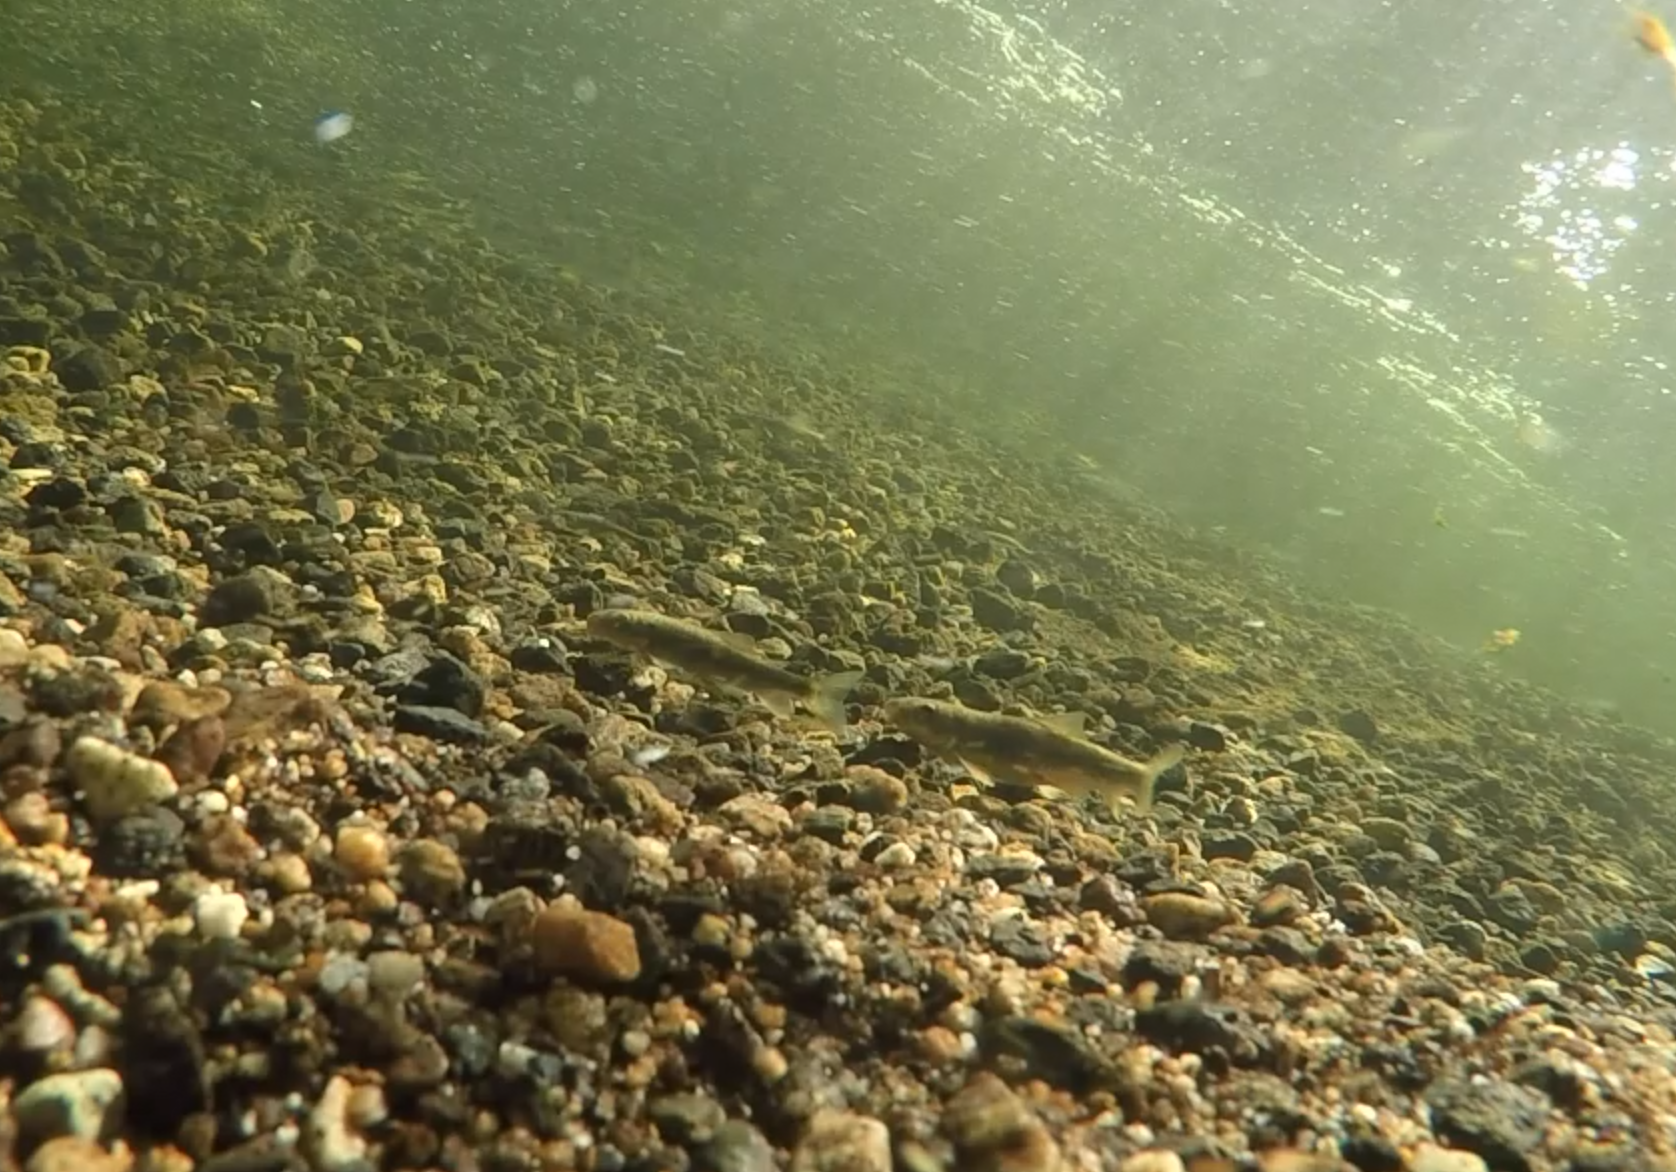
\includegraphics[scale=.5]{reallygoodcrop}

\end{figure}
\end{document}
